
% Copyright (c) 2015 - 2020 Mario Mlačak, mmlacak@gmail.com
% Licensed and published as Public Domain work.

% Hemera's Dawn chapter ===============================================
\chapter*{Hemera's Dawn}
\addcontentsline{toc}{chapter}{Hemera's Dawn}

\begin{flushright}
\parbox{0.8\textwidth}{
\emph{Then assuredly the world was made, not in time, but simultaneously with time. \\
\hspace*{\fill}{\textperiodcentered \textperiodcentered \textperiodcentered \hspace*{0.2em} St. Augustine} } }
\end{flushright}

\noindent
Hemera's Dawn is chess variant which is played on 20 x 20 board, with
darkish red-brown and grey fields and pure red and bright yellow pieces.
Star colors are bright blue and white. In algebraic notation, columns
are enumerated from 'a' to 't', and rows are enumerated from '1' to '20'.
A new piece is introduced, Centaur.

\clearpage % ..........................................................
% Centaur *************************************************************

\section*{Centaur}
\addcontentsline{toc}{section}{Centaur}

\noindent
\begin{wrapfigure}[11]{l}{0.4\textwidth}
\centering
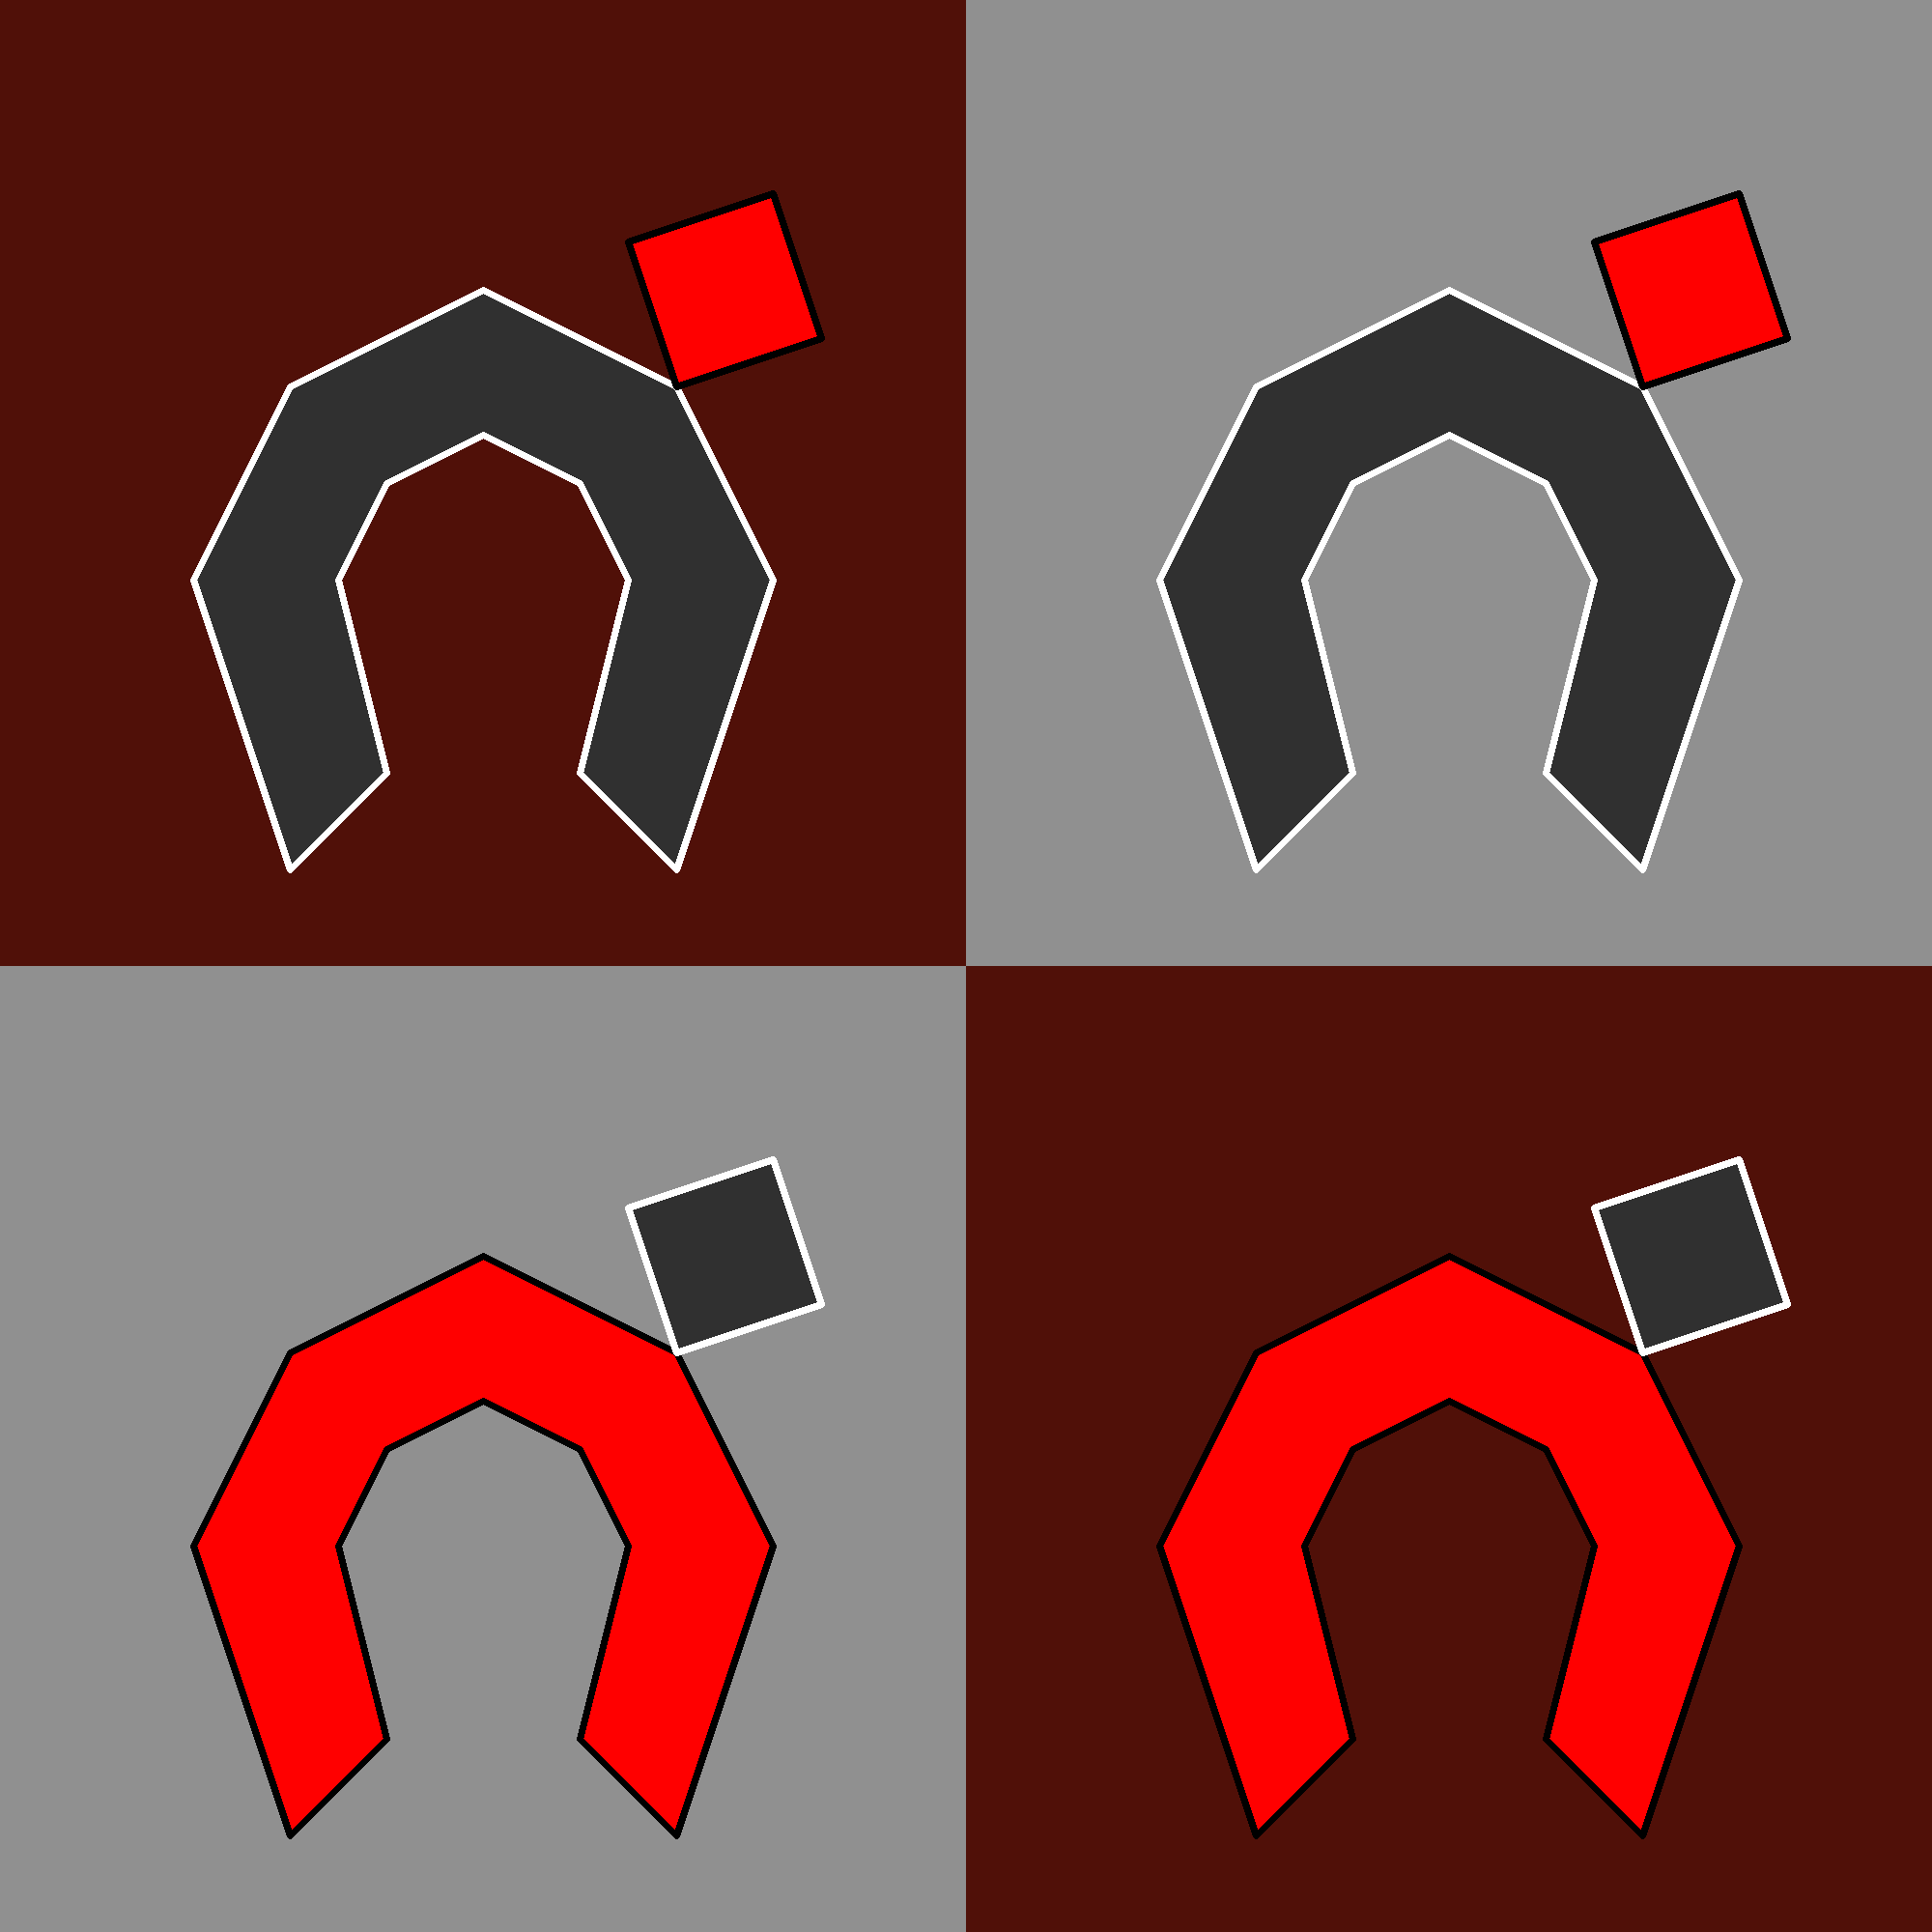
\includegraphics[width=0.4\textwidth, keepaspectratio=true]{pieces/12_centaur.png}
\caption{Centaur}
\label{fig:12_centaur}
\end{wrapfigure}
Centaur is similar to Unicorn, only it can continue its' jumpy movement
in two chosen directions until another piece is encountered, or it runs
out of a chessboard.

The two directions are chosen freely on first and second jump. Once both
long and short jump directions are determined, Centaur has to follow them
in all subsequent steps, for the remainder of that ply.

For Centaur's ply to be legal, all steps must end up on the chessboard.

In algebraic notation symbol for Centaur is ’C’.

% \vspace*{0.05\textheight}
\noindent
\begin{wrapfigure}{l}{0.4\textwidth}
\centering
\includegraphics[width=0.4\textwidth, keepaspectratio=true]{pieces/star/14_hemera_s_dawn.png}
\caption{Star}
\label{fig:star/14_hemera_s_dawn}
\end{wrapfigure}
Star colors in this variant are different to colors of light and dark pieces.

\clearpage % ..........................................................
% Movement ------------------------------------------------------------

% \vspace{7\baselineskip}
\subsection*{Movement}
\addcontentsline{toc}{subsection}{Movement}

\noindent
\begin{wrapfigure}{l}{0.4\textwidth}
\centering
\includegraphics[width=0.35\textwidth, keepaspectratio=true]{examples/14_hd/scn_hd_01_centaur_same_color.png}
\caption{Centaur short jump}
\label{fig:scn_hd_01_centaur_same_color}
\end{wrapfigure}
On fields with the same color as Centaur, it can move exactly the
same way Knight does.

\clearpage % ..........................................................

\noindent
\begin{figure}[!h]
% \begin{figure}[!t]
\includegraphics[width=1.0\textwidth, keepaspectratio=true]{examples/14_hd/scn_hd_02_centaur_opposite_color.png}
\caption{Centaur long jump}
\label{fig:scn_hd_02_centaur_opposite_color}
% \centering
\end{figure}

On fields in opposite color, Centaur can jump much longer, exactly the
same way Unicorn does. Again, just as Knight (and Unicorn), Centaur is
not hampered by surrounding pieces. Only own pieces on marked (i.e. step)
fields can prevent Centaur to move, opponent's pieces could be captured.

For comparison, Knight's step-fields are also numbered (grey).

\clearpage % ..........................................................

\noindent
\begin{figure}[!h]
% \begin{figure}[!t]
\includegraphics[width=1.0\textwidth, keepaspectratio=true]{examples/14_hd/scn_hd_03_centaur_multi_step.png}
\caption{Centaur multi-step move}
\label{fig:scn_hd_03_centaur_multi_step}
% \centering
\end{figure}

On first two jumps, Centaur can choose freely any direction (blue). After
two directions are chosen, Centaur for the rest of a ply has to follow
them (green), e.g. after reaching field 6, it cannot move to any 7a to 7g
fields (red). \\
Here, step-fields are numbered 1 to 11, they are also capture-fields. Light
Centaur could capture dark Bishop, but is prevented from moving any further
(grey). Pieces on all other fields are ignored (Pawns).

\clearpage % ..........................................................

\subsubsection*{Out of board steps}
\addcontentsline{toc}{subsubsection}{Out of board steps}

\vspace*{-0.05\textwidth}
\noindent
\begin{figure}[!h]
% \begin{figure}[!t]
\includegraphics[width=1.0\textwidth, keepaspectratio=true]{examples/14_hd/scn_hd_04_centaur_off_board.png}
\caption{Centaur off-board steps}
\label{fig:scn_hd_04_centaur_off_board}
% \centering
\end{figure}

Here, light grey fields are virtual fields extending existing chessboard.
It's illegal to step outside chessboard, and all subsequent steps are also
illegal. That means, Centaur cannot reach fields 1 and 2 from starting
position with selected directions, even though it would end movement on the
chessboard.

\clearpage % ..........................................................
% ------------------------------------------------------------ Movement

\subsection*{Activating Wave}
\addcontentsline{toc}{subsection}{Activating Wave}

\vspace*{-1.0\baselineskip}
\noindent
\begin{figure}[!h]
% \begin{figure}[!t]
\includegraphics[width=1.0\textwidth, keepaspectratio=true]{examples/14_hd/scn_hd_05_wave_activation_by_centaur.png}
\caption{Wave activation by Centaur}
\label{fig:scn_hd_05_wave_activation_by_centaur}
% \centering
\end{figure}

Wave activated by Centaur moves \hyperref[fig:scn_hd_03_centaur_multi_step]{the same way},
i.e. on first two jumps, Wave has to choose long and short step (blue). After two directions
are chosen, Wave for the rest of a ply has to follow them (green), and cannot change mid-ply
(red).

Light Wave could also activate dark Wave on a step-field, pieces on all other fields are
ignored (Pawns).

\clearpage % ..........................................................

\subsubsection*{Out of board steps}
\addcontentsline{toc}{subsubsection}{Out of board steps}

\vspace*{-1.2\baselineskip}
\noindent
\begin{figure}[!h]
% \begin{figure}[!t]
\includegraphics[width=1.0\textwidth, keepaspectratio=true]{examples/14_hd/scn_hd_06_wave_activated_by_centaur_off_board.png}
\caption{Wave off-board steps}
\label{fig:scn_hd_06_wave_activated_by_centaur_off_board}
% \centering
\end{figure}

Again, light grey fields are virtual fields extending existing chessboard.
Wave activated by Centaur can step outside of a board, as long as its' ply
ends on a board, just like
\hyperref[fig:scn_mv_26_wave_off_board]{Wave activated by Unicorn}. Here,
step-fields 1 and 2 are reachable by Wave, even though it stepped outside
of the board. It is illegal for any piece, including Wave, to end its' ply
outside of a board.

\clearpage % ..........................................................

\subsection*{Teleporting Wave}
\addcontentsline{toc}{subsection}{Teleporting Wave}

\vspace*{-1.2\baselineskip}
\noindent
\begin{figure}[!h]
% \begin{figure}[!t]
\includegraphics[width=1.0\textwidth, keepaspectratio=true]{examples/14_hd/scn_hd_07_wave_teleport.png}
\caption{Wave off-board teleporting}
\label{fig:scn_hd_07_wave_teleport}
% \centering
\end{figure}

Activation by Centaur and following teleportation of Wave is
\hyperref[fig:scn_n_07_teleport_wave_init]{exactly the same as if activated by Unicorn},
except Wave can now carry more than 1 momentum, because Centaur's ply can be
longer than just 1 step.

\clearpage % ..........................................................
% ************************************************************* Centaur
% \clearpage % ..........................................................

\section*{Promotion}
\addcontentsline{toc}{section}{Promotion}

Promotion is non enforced, delayed variety, i.e. it's the same as in
\hyperref[sec:Age of Aquarius/Promotion]{previous chess variant}, Age of Aquarius.

Promotion in this variant is polygamous, more than one Queen in the same color
can be present on chessboard at any given time.

\clearpage % ..........................................................

\section*{Rush, en passant}
\addcontentsline{toc}{section}{Rush, en passant}

\noindent
\begin{wrapfigure}{l}{0.4\textwidth}
\centering
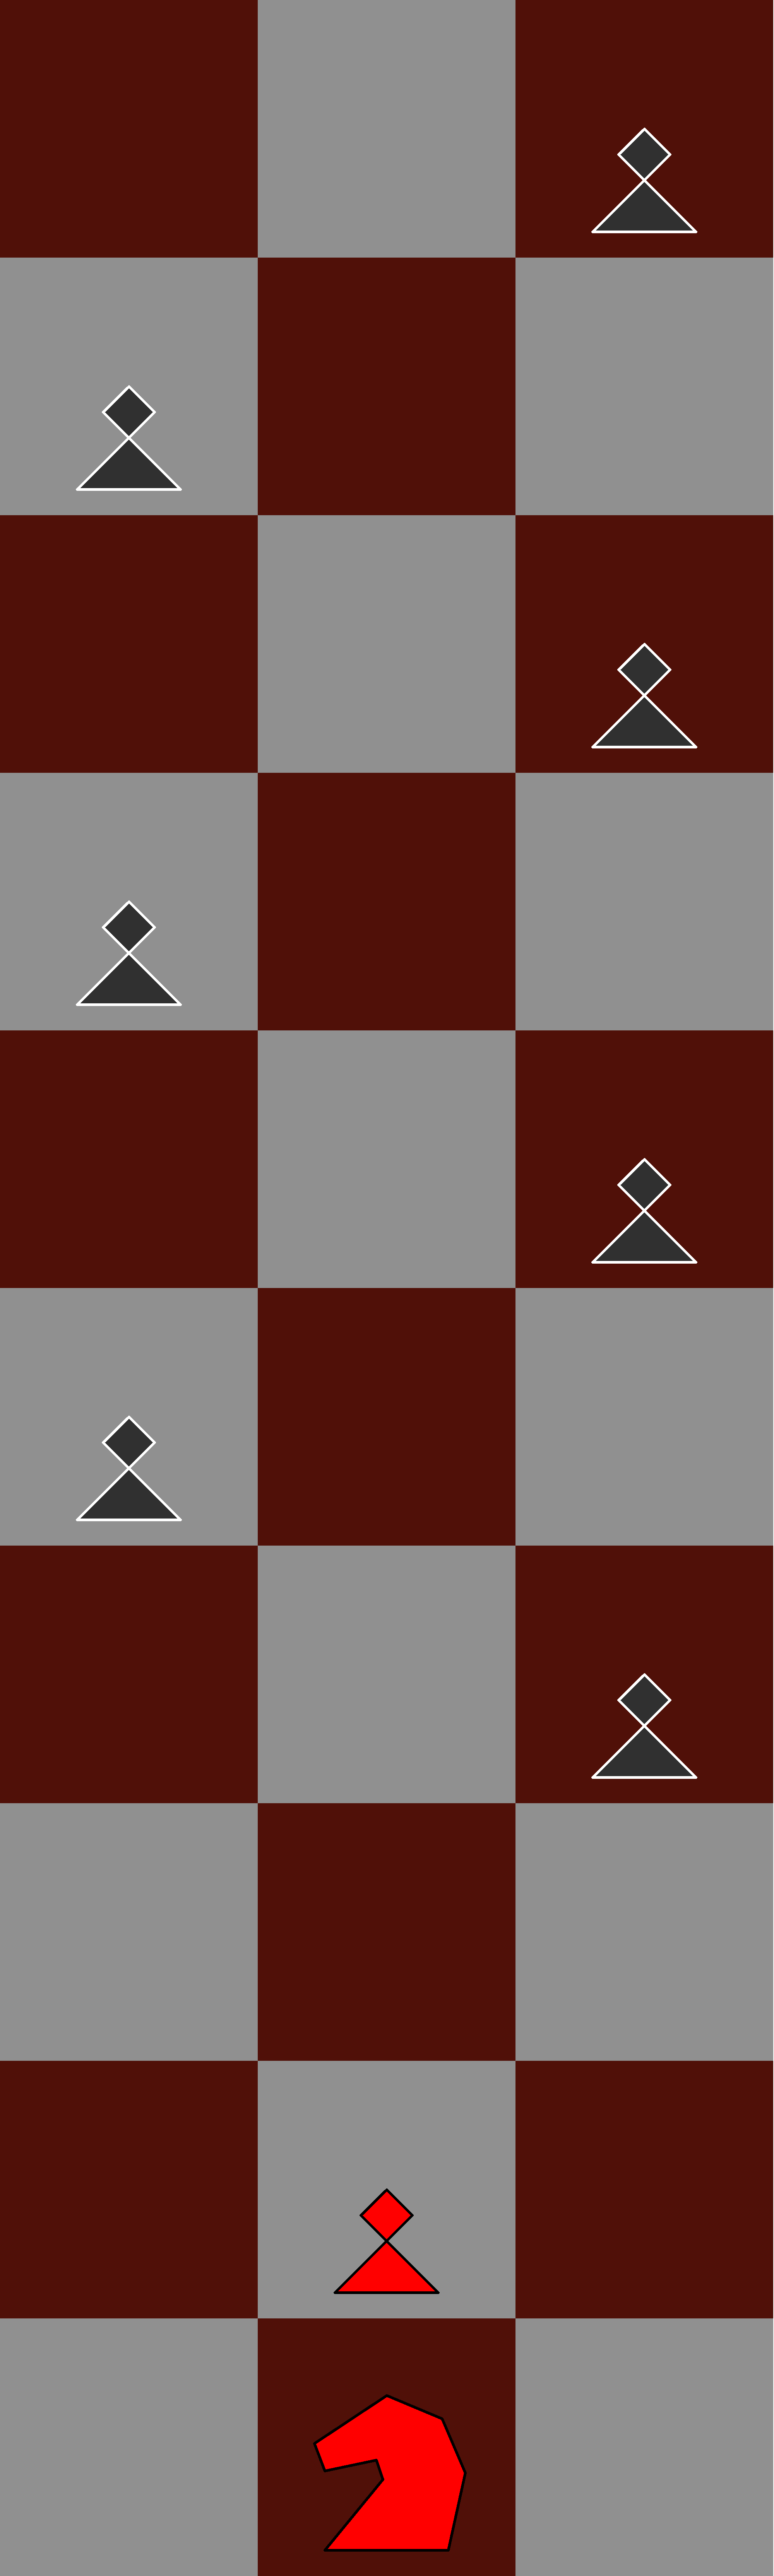
\includegraphics[width=0.35\textwidth, keepaspectratio=true]{en_passants/14_hemera_s_dawn_en_passant.png}
\caption{En passant}
\label{fig:14_hemera_s_dawn_en_passant}
\end{wrapfigure}
Rush and en passant are identical to those in Classic Chess, only difference
is that Pawn can now move longer on initial turn, up to 8 fields in this
variant.

\clearpage % ..........................................................

\section*{Castling}
\addcontentsline{toc}{section}{Castling}

Castling is the same as in Classical Chess, only difference is that King can move between 2 and 7 fields across.
All other constraints from Classical Chess still applies.

\noindent
\begin{figure}[!h]
% \begin{figure}[!t]
\includegraphics[width=1.0\textwidth, keepaspectratio=true]{castlings/14_hd/hemera_s_dawn_castling.png}
\caption{Castling}
\label{fig:hemera_s_dawn_castling}
% \centering
\end{figure}

In example above, all valid King's castling moves are numbered.

\noindent
\begin{figure}[!h]
% \begin{figure}[!t]
\includegraphics[width=1.0\textwidth, keepaspectratio=true]{castlings/14_hd/hemera_s_dawn_castling_right_03.png}
\caption{Castling short right}
\label{fig:hemera_s_dawn_castling_right_03}
% \centering
\end{figure}

In this example King was castling short to the right. Initial King's position is marked with "K".
After castling is finished, right Rook ends up at field immediately left to the King.

\clearpage % ..........................................................

\section*{Initial setup}
\addcontentsline{toc}{section}{Initial setup}

Compared to initial setup of Nineteen, Centaur is inserted between Knight and Wave
symmetrically, on both sides of chessboard. This can be seen in the image below:

\noindent
% \begin{figure}[t]
\begin{figure}[h]
\includegraphics[width=1.0\textwidth, keepaspectratio=true]{boards/14_hemera_s_dawn.png}
\caption{Hemera's Dawn board}
\label{fig:14_hemera_s_dawn}
% \centering
\end{figure}

\clearpage % ..........................................................
% =============================================== Hemera's Dawn chapter
